\part{Vision}


\section{Conics and quadrics}

\subsection{Ellipses}
The general quadratic equation of a conic is: $Ax^2 + Bxy + Cy^2 + Dx + Ey + F = 0 $

It can be written in the homogeneous form:
\begin{equation}
(x~~y~~1) \left[\begin{array}{ccc}
     A & B/2 & d/2  \\
     B/2 & C & E/2 \\
     D/2 & E/2 & F
\end{array}\right] 
\left( \begin{array}{c}
     x  \\
     y \\
     1
\end{array} \right)
= 0
\end{equation}
In 2D projective geometry, all conics are equivalent under a projective transformation.

An ellipse is a specific form of conic and has the equation:
\begin{equation}
\frac{x^2}{a^2} + \frac{y^2}{b^2} = 1
\end{equation}

\subsubsection{Euclidean matrix form}
\begin{equation}
    (X - C)^T A (X - C) = 1
\end{equation}
$C$ is the ellipse center and $A$ is a 2x2 symmetric matrix defining its shape. The eigen vectors of $A$ are the two axes and their corresponding eigen values give $1/a^2$ and $1/b^2$.

It is possible to extract the rotation part out of $A$:
\begin{equation}
(X - C)^T {}^{e}R_{w}^T \left[ \begin{array}{cc}
    1/a^2 & 0 \\
    0 & 1/b^2
\end{array}
\right] {}^{e}R_{w} (X - C) = 1
\end{equation}

\subsubsection{Homogeneous form}
\begin{equation}
    X^T T_{-C}^T
    {}^{e}R_{w}^T
    \left[ \begin{array}{ccc}
    1/a^2 & 0 & 0\\
    0 & 1/b^2 & 0\\
    0 & 0 & -1
    \end{array}\right]
    {}^{e}R_{w}
    T_{-C}
    X = 0
\end{equation}

where $T_{-C} = \left[\begin{array}{ccc}
    1&0&-C_x \\
    0&1&-C_y \\
    0&0&1
    \end{array}\right]$ is a translation to move the ellipse center to~(0, 0).

This gives a complete homogeneous equation:
\begin{equation}
    X^T C X = 0
\end{equation}
where $C$ is a 3x3 symmetric matrix defined up to a scale (6 elements for only 5 parameters because of the scale).

\subsubsection{Dual form}
It defines the ellipse by tangent lines instead of points. It satisfies:
\begin{equation}
    l^T C^* l = 0
\end{equation}

where $C^*$ is the adjointe matrix of $C$ and we have $C^* \sim C^{-1}$

\subsubsection{Decompose an ellipse}
This show how to decompose an ellipse into: half-axes, orientation and center.
Input: $C$ the matrix of the dual conic

\begin{enumerate}
\item Normalize by minus the last element $C/-C[2, 2]$ to force C[2, 2] = -1
\item $c = -C[:2, 2]$ is the center of the ellipse
\item Apply translation of minus the center to get the ellipse centered. $C_{centered} = T_{-c} C T_{-c}^T $
\item Enforce symmetry: $C_{centered} = 0.5 (C_{centered}+C_{centered}^T)$
\item Compute eigen decomposition $D, R = eig(C_{centered}[:2, :2])$
\item $a, b = sqrt(abs(D))$, $orientation = R$ and $center = c$
\end{enumerate}

\subsubsection{Fit an ellipse}
An ellipse have 5 degrees of freedom (3x3 symmetric matrix: 6 parameters -1 for the scale).

Each point gives one equation, so we need at least 5 points.
\begin{equation}
    \left[
    \begin{array}{cccccc}
    x_i^2 & x_i y_i & y_i^2 & x_i & y_i & 1  \\
    \vdots &\vdots &\vdots &\vdots &\vdots &\vdots 
    \end{array}
    \right]
    \left[\begin{array}{c}
        a \\ b \\ c \\ d \\ e \\ f
    \end{array} \right]
    = 0
\end{equation}

solve this homogeneous system $Ax=0$ with SVD. The last row of $Vt$ gives the best estimation.


\subsection{Ellipsoids}

Ellipsoids are quadrics with the following type of equation:
\begin{equation}
    \frac{x^2}{a^2} + \frac{y^2}{b^2} + \frac{z^2}{c^2} = 1
\end{equation}

\subsubsection{Euclidean matrix form}
Similar to the ellipse case, the general Euclidean form of an ellipsoid is:
\begin{equation}
    (X - C)^T A (X - C) = 1
\end{equation}
$C$ is the ellipse center and $A$ is a 3x3 symmetric matrix defining its shape. The eigen vectors of $A$ are the three axes and their corresponding eigen values give $1/a^2$, $1/b^2$ and $1/c^2$.

Again, it is possible to extract the rotation out of $A$:

\begin{equation}
(X - C)^T {}^{e}R_{w}^T \left[ \begin{array}{ccc}
    1/a^2 & 0 & 0 \\
    0 & 1/b^2 & 0 \\
    0 & 0 & 1/c^2
\end{array}
\right] {}^{e}R_{w} (X - C) = 1
\end{equation}


\subsubsection{Homogeneous form}
\begin{equation}
    X^T T_{-C}^T
    {}^{e}R_{w}^T
    \left[ \begin{array}{cccc}
    1/a^2 & 0 & 0 & 0\\
    0 & 1/b^2 & 0 & 0\\
    0 & 0 & 1/c^2 & 0\\
    0 & 0 & 0 & -1
    \end{array}\right]
    {}^{e}R_{w}
    T_{-C}
    X = 0
\end{equation}

where $T_{-C} = \left[\begin{array}{cccc}
    1&0&0&-C_x \\
    0&1&0&-C_y \\
    0&0&1&-C_z \\
    0&0&0&-1
    \end{array}\right]$ is a translation to move the ellipsoid center to~(0, 0, 0).

This gives a complete homogeneous equation:
\begin{equation}
    X^T Q X = 0
\end{equation}

where $Q$ is a 4x4 symmetric matrix defined up to a scale (10 elements for only 9 parameters because of the scale).

\subsubsection{Dual form}
It defines the ellipsoid by tangent planes instead of points. It satisfies:
\begin{equation}
    l^T Q^* l = 0
\end{equation}

where $Q^*$ is the adjointe matrix of $Q$ and we have $Q^* \sim Q^{-1}$


\subsubsection{Decompose an ellipsoid}
This show how to decompose an ellipsoid into: half-axes, orientation and center.
Input: $Q$ the matrix of the dual quadric
\begin{enumerate}
\item Normalize by minus the last element $Q/-Q[3, 3]$ to force Q[3, 3] = -1
\item $c = -Q[:3, 3]$ is the center of the ellipsoid
\item Apply translation of minus the center to get the ellipsoid centered. $Q_{centered} = T_{-c} Q T_{-c}^T $
\item Enforce symmetry: $Q_{centered} = 0.5 (Q_{centered}+Q_{centered}^T)$
\item Compute eigen decomposition $D, R = eig(Q_{centered}[:3, :3])$
\item $a, b, c = sqrt(abs(D))$, $orientation = R$ and $center = c$
\end{enumerate}

\section{2D Transformations}

\begin{tabular}{|c|c|c|c|}
 \hline
  Transformation & degrees of freedom & matrix & invariants \\
  \hline
  Projective & 8 dof & 
  $\left[\begin{array}{ccc}
       h_{11}&h_{12}&h_{13}  \\
       h_{21}&h_{22}&h_{23}  \\
       h_{31}&h_{32}&h_{33}  \\
    \end{array}\right]$ & 
    \begin{minipage}[t]{0.4\textwidth}
    \begin{itemize}
        \item lines (collinearity)  
        \item cross ratios (ratio of ratio)
    \end{itemize}
    \end{minipage}
    \\
    \hline
    
      Affine & 6 dof & 
  $\left[\begin{array}{ccc}
       a_{11}&a_{12}&t_{x}  \\
       a_{21}&a_{22}&t_{y}  \\
       0 & 0 & 1  \\
    \end{array}\right]$ & 
    \begin{minipage}[t]{0.4\textwidth}
    \begin{itemize}
        \item parallelism
        \item centroid
        \item line at infinity
    \end{itemize}
    \end{minipage}
    \\
    \hline
    
    Similarity & 4 dof & 
  $\left[\begin{array}{ccc}
       sr_{11}&sr_{12}&t_{x}  \\
       sr_{21}&sr_{22}&t_{y}  \\
       0 & 0 & 1  \\
    \end{array}\right]$ & 
    \begin{minipage}[t]{0.4\textwidth}
    \begin{itemize}
        \item angles
        \item ratio of length
        \item ratio of areas
    \end{itemize}
    \end{minipage}
    \\
    \hline
    
       Isometry (Euclidean) & 3 dof & 
  $\left[\begin{array}{ccc}
       r_{11}&r_{12}&t_{x}  \\
       r_{21}&r_{22}&t_{y}  \\
       0 & 0 & 1  \\
    \end{array}\right]$ & 
    \begin{minipage}[t]{0.4\textwidth}
    \begin{itemize}
        \item length
        \item angles
    \end{itemize}
    \end{minipage}
    \\
    \hline
\end{tabular}

\textbf{\underline{Note:}}

A similarity transform can be decomposed as a rotation $\theta$ and a non-uniform scaling $D$ with a certain orientation $\phi$:  $S = R(\theta)R(-\phi)DR(\phi)$

The group of invertible nxn matrices is the \textit{General Linear Group}.

The \textit{Projective Linear Group} is a subgroup of the matrices which are equivalent by a scalar factor.


\subsection{Topology of the projective plane}
Any point can be normalized such that: $x_1^2 + x_2^2 + x_3^2 = 1$.
Such point lies on the unit sphere $S^2$ in $R^3$
There is a 2-to-1 correspondence between $S^2$ and $P^2$.
Opposite points on the sphere represent the same point. Any two points on the sphere lies on a single great circle which correspond to the line between the two points. Any two great circles intersect into a single points (in fact 2 opposite points which represent the same point).

\subsubsection{Homogenous representation of points}
The homogeneous representation of a point is :
\begin{equation}
    \textbf{p} \sim \left(\begin{array}{c}
        \bar{p}\\1
    \end{array}\right)
    =
    \left(\begin{array}{c}
        x\\y\\1
    \end{array}\right)
\end{equation}

\textbf{P-normalization}
The mapping $R^2 \rightarrow P^2$ has an inverse mapping obtained by normalization.
\begin{equation}
    \textbf{x} = \left(\begin{array}{c}
        x_1 \\ x_2 \\ x_3
    \end{array}\right)
\end{equation}
and
\begin{equation}
    \textbf{x} \sim \left(\begin{array}{c}
        x_1 / x_3 \\ x_2 / x_3 \\ 1
    \end{array}\right)
\end{equation}


\subsubsection{Homogenous representation of lines}
Equation of a line in 2D: $l_1x + l_2y - \Delta = 0$

In homogeneous coordinates the line becomes:
\begin{equation}
    \textbf{l} \sim \left(\begin{array}{c}
        l_1 \\ l_2 \\ -\Delta
    \end{array}\right)
\end{equation}
In the canonical form, we assume $l_1^2 + l_2^2 = 1$ and $\Delta \ge 0$.
The previous equation becomes: $x^Tl=0$.


\textbf{D-normalization}
\begin{equation}
    \textbf{l} = \left(\begin{array}{c}
        \beta_1 \\ \beta_2 \\ \beta_3
    \end{array}\right)
\end{equation}

To go back to the canonical form, we do:
\begin{equation}
    \textbf{l}\sim \frac{-sign(\beta_3)}{\sqrt{\beta_1^2+\beta_2^2}} \left(\begin{array}{c}
        \beta_1 \\ \beta_2 \\ \beta_3
    \end{array}\right)
    = \left(\begin{array}{c}
        l_1 \\ l_2 \\ -\Delta
    \end{array}\right)
\end{equation}



\section{Gaussian and $\chi^2$ distributions}
\subsubsection{Gaussian probability distribution}
Given a vector $X$ of random variables $x_i$ for $i=1,\dots,N$, with mean $\bar{X} = E[X]$, and $\Delta_X = X - \bar{X}$, the covariance matrix $\Sigma$ is a NxN matrix given by

\begin{equation}
    \Sigma = E[\Delta_X \Delta_X^T]
\end{equation}

so that $\Sigma_{ij}=E[\Delta_{x_i}\Delta_{y_i}]$. The diagonal elements of $\Sigma$ are the variances of the individual variables $x_i$, and the off-diagonal elements are the cross-variances values.
In non-degenerate cases, where $\Sigma$ is positive-definite and thus invertible, the multivariate Gaussian distribution is
\begin{equation}
P(X)=\frac{1}{(2\pi)^{N/2}|\Sigma|^{1/2}} e^{-\frac{1}{2}(X-\bar{X})^T \Sigma^{-1} (X-\bar{X})}
\end{equation}

where $|\Sigma|$ is the determinant of $\Sigma$.

In the case where $\Sigma$ is just a diagonal matrix with a unique scalar term on the diagonal, $\Sigma=\sigma^2 I$, the distribution is called an \textit{isotropic Gaussian distribution}.

\subsubsection{Mahalanobis distance}

It is defined as:
\begin{equation}
    \norm{X - Y}_{Sigma}=\sqrt{(X-Y)^T \Sigma^{-1} (X-Y)}
\end{equation}{}

where $\Sigma$ is a positive definite matrix. This defines a metrix on $R^N$.
We can see that the Gaussian distribution is equivalent (without the normalization terms) to 

\begin{equation}
    P(X) \approx e^{-\frac{\norm{X-\bar{X}}_{\Sigma}^{2}}{2}}
\end{equation}{}

\subsubsection{Change of coordinates}
Since $\Sigma$ is symmetric and positive-definite, it may be rewritten as $\Sigma=U^T D U$, where $U$ is an orthogonal matrix and $D=(\sigma_1^2, \sigma_2^2, \dots, \sigma_N^2)$ is diagonal.

This shows that a general Gaussian PDF can be changed into an \textit{isotropic Gaussian distribution} with an orthogonal change of coordinates $X^\prime = UX$ and a scaling $\sigma_i$ of each component.
This also show that Euclidean distance and Mahalanobis distances are equivalent under a change of coordinates.

\subsection{$\chi^2$ distribution}

The $\chi_n^2$ distribution is the distribution of the sum of squares of $n$ independant Gaussian random variables. For a Gaussian random vector $v$, the value ${(v-\bar{v})^T \Sigma^{-1} (v-\bar{v})}$ satisfies a $\chi_n^2$ distribution, where $n$ is the dimension of $v$.



\section{Algorithm evaluation and error analysis}
\underline{Convention}
$x$ represents a measured image point.
Estimated quantities are represented with a hat, $\hat{x}$ or $\hat{H}$.
True values are represented with a bar, $\bar{x}$ or $\bar{H}$.

In the following subsections, we treat the problem of estimating a projective transformation between 2D points.

\subsection{Error in one image}

Suppose the points in the first image are noise-free $x_i = \bar{x}_i$ and points in the second image $x^\prime_i$ have a Gaussian noise. After estimating the transform $\hat{H}$, we can compute a \textit{residual error} which gives the average difference between the noisy input data $x^\prime_i$ and the 
estimated points $\hat{x}^\prime_i = \hat{H}\bar{x}_i$

\begin{equation}
    \epsilon_{res} = \sqrt{\left( \frac{1}{2n}\sum_{i=1}^{n} d(x^\prime_i,\hat{x}^\prime_i)^2 \right)}
\end{equation}{}

In case of only 4 points, the estimated homography will perfectly fit the noisy input data and thus the residual error will be 0. However, this estimation will not be very close approximation to the noise-free values.
With more than 4 points, the residual error will increase, but the estimated model will agree more and more with the noise-free true values.

\subsection{Error in both images}
In case of errors in both images, the residual error becomes

\begin{equation}
    \epsilon_{res} = \frac{1}{\sqrt{4n}} \sqrt{\sum_{i=1}^{n} d(x_i, \hat{x}_i)^2 + \sum_{i=1}^{n} d(x^\prime_i, \hat{x}^\prime_i)^2}
\end{equation}{}

where $\hat{x}_i$ and $\hat{x}_i^\prime$ are estimated points such that $\hat{x}_i = \hat{H} \hat{x}_i^\prime$.


\subsection{Optimal estimators (MLE)}
Maximum Likelyhood Estimator (MLE) gives a theoretical optimal solution and any other algorithm should be compared to it.
A general estimation problem is with function $f$ from $R^M$ to $R^N$ where $R^M$ is a parameter space and $R^N$ is a space of measurements. Consider a point $\bar{X}$ from the measurement space for which there exists a point $\bar{P}$ in the parameters space such that $f(\bar{P}) = \bar{X}$. In case of homography between 2 sets of $n$ points, $\bar{X}$ contains its $N=2n$ coordinates and $\bar{P}$ contains the 8 or 9 parameters of the homography.

Let $X$ be a measurement chosen according to an isotropic Gaussian distribution of mean $\bar{X}$ and total variance $N\sigma^2$ (this is the sum of the variance of each component = trace of the covariance matrix).

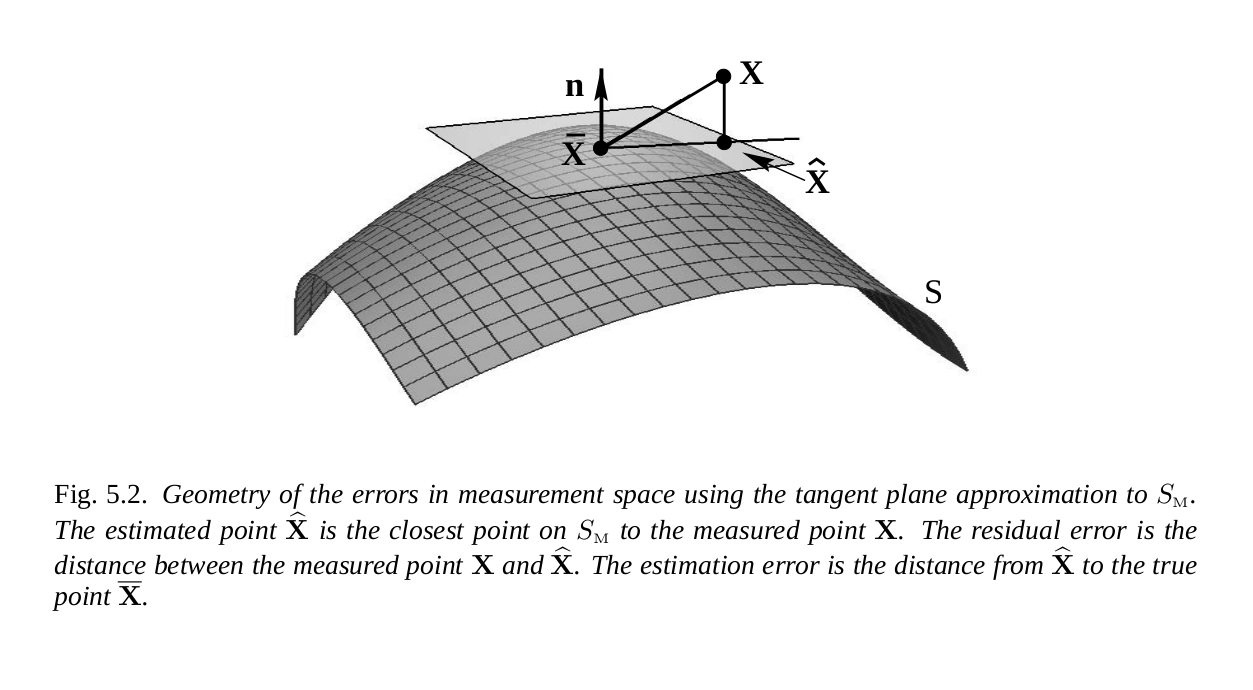
\includegraphics[scale=0.25]{content/MLE.png}

As the value of the parameter vector $P$ varies in a neighbourhood of $\bar{P}$, the values of $f(P)$ traces out a surface $S_m$ in $R^N$ through point $\bar{X}$. This surface is a sub-manifold of $R^N$ and has dimension $d$, the number of essential parameters (= nb of degrees of freedom or minimum number of parameters). The ML estimate $\hat{X}$ is the point on the curve which is the closest to the measurement point $X$.

If we assume that in a neighbourhood of $\bar{X}$, the surface is planar, this ML estimate is the orthogonal projection of $X$ onto the plane.
The residual error corresponds to the distance between $X$ and $\hat{X}$. Its distribution is the projection of the distribution of the Gaussian distribution variable on the $N-d$-dimensional normal of the plane.
The estimator error corresponds to the distance between $\bar{X}$ and $\hat{X}$. Its distribution is projection of the distribution of the Gaussian random variable onto the $d$-dimensional plane.

With this its possible to compute the \textbf{expected residual errors} and the \textbf{expected estimator error}.

\subsection{Covariance of the estimation}

We saw in the previous subsection that the achievable residual error and estimation error depends only on the number of points correspondence and their accuracy. However, the confidence of the estimation (its covariance) depends also on the configuration off the points. For example, if we take 4 points almost collinear, the behaviour of the transformation along the perpendicular dimension cannot be accurately estimated. This uncertainty is captured in the \textit{covariance matrix}.

\subsubsection{Forward propagation of covariance (linear case)}

Let $v$ be a random vector in $R^M$ with mean $\bar{v}$ and covariance matrix $\Sigma$ and suppose that $f : R^M \rightarrow R^N$ is an affine matrix defined by $f(v) = f(\bar{v}) + A(v - \bar{v})$.
Then $f(v)$ is a random variable with mean $f(\bar{v})$ and covariance matrix $A\Sigma A^T$.


